% File naaclhlt2010.tex
% Contact: nasmith@cs.cmu.edu
\documentclass{llncs}
\usepackage{times}
\usepackage{url}
\usepackage{latexsym}
\usepackage{amsmath}
\usepackage{multirow}
\usepackage{url}
%\DeclareMathOperator*{\argmax}{arg\,max}
%\setlength\titlebox{6.5cm}    % Expanding the titlebox


\usepackage{arabtex}
\usepackage{amssymb}
\usepackage{caption}
\usepackage{epsfig}
\usepackage{subfigure}
\usepackage{color}
\usepackage{rotate}
\usepackage{rotating}
%\usepackage{amsthm}
%\usepackage{booktabs}

\usepackage{relsize}
%\usepackage{fancyvrb}
\usepackage[colorlinks=false,draft]{hyperref}
%\usepackage[colorlinks=false]{hyperref}

%\allowarab{\fbox}
\usepackage{utf8}
\setarab
\fullvocalize
\transtrue
\arabtrue


%\newcommand{\CharCodeIn}[1]{`\CodeIn{#1}'}
\newcommand{\true}{\ensuremath{\mathit{true}}}
\newcommand{\false}{\ensuremath{\mathit{false}}}

\newcommand{\cci}[1]{{\small\texttt{#1}}}
\newcommand{\chci}[1]{\cci{#1}}

\newcommand{\frl}[1]{\fbox{\RL{#1}}} 
\newcommand{\noArRL}[1]{\arabfalse\RL{#1}\arabtrue} 
\newcommand{\noTrRL}[1]{\transfalse\RL{#1}\transtrue} 
\newcommand{\noTrnoVocRL}[1]{\transfalse\novocalize\noTrRL{#1}\vocalize\transtrue}  
\newcommand{\noVocRL}[1]{\transtrue\novocalize\RL{#1}\vocalize}  
\newcommand{\utfRL}[1]{\setcode{utf8} \RL{#1} \setcode{standard}}
\newcommand{\noTrnoVocutfRL}[1]{\setcode{utf8} \transfalse\novocalize\RL{#1}\vocalize \transtrue \setcode{standard}}
\newcommand{\noTrutfRL}[1]{\setcode{utf8} \transfalse\RL{#1}\transtrue \setcode{standard}}
\newcommand{\noArutfRL}[1]{\setcode{utf8} \arabfalse \RL{#1} \arabtrue \setcode{standard}} 

%\title{Instructions for NAACL HLT 2010 Proceedings\Thanks{This...}}
\title{Arabic Entity Graph Extraction using Morphology, Finite State Machines, and Graph Transformations}

\author{ Jad Makhlouta\inst{1} \and
    Fadi Zaraket\inst{1} \and 
Hamza Harkous\inst{1} }
\institute{ American University of Beirut \\
  \email{ \{jem04, fz11, hhh20\}@aub.edu.lb } }
\date{}

\begin{document}
\maketitle

\begin{abstract}
Research on automatic recognition of named entities
%events and relations amongst them 
from Arabic text uses techniques that work well for the 
Latin based languages such as local grammars, 
statistical learning models, pattern matching, 
and rule-based techniques. 
These techniques boost their results by using application 
specific 
corpora, parallel language corpora,
and morphological stemming analysis. 
We propose a method for extracting entities, events, 
and relations amongst them
from Arabic text using 
a hierarchy of finite state machines driven by morphological 
features such as part of speech and gloss tags,
and graph transformation algorithms. 
We evaluated our method on two natural language processing 
applications.
We automated the extraction of narrators and 
narrator relations from 
several corpora of Islamic narration books. 
We automated the extraction of genealogical family trees 
from Biblical texts. 
%Finally, we automated locating and extracting
%individual biographies from historical biography books.
In all applications, our method reports high precision and recall
and learns lemmas about phrases that improve results. 
\end{abstract}


\section{Introduction}
Named entity recognition (NER) is harder for Arabic text than 
it is for Latin. 
Arabic does not have upper case letters which distinguish the 
start and end of named entities (NE).
Arabic is morphologically rich, 
more ambiguous than Latin languages,
and its short vowels are frequently omitted~\cite{Debili1998}.

Industrial tools that perform NE extraction for Arabic exist~\cite{Sak09,IdentiFinder,basis:06,ANEE:07},
but little is said about the techniques behind them and no formal evaluation of the tools exist. 
Researchers proposed and evaluated 
local grammars with morphological stemming~\cite{ZAGHOUANI10,Traboulsi:09},
rule-based systems powered with local grammars~\cite{ShaalanR09} 
and stop words ~\cite{Abuleil04},
statistical analysis boosted with Arabic-English parallel corpora~\cite{BenajibaZDR10}, 
statistical analysis boosted with task specific gazetteers~\cite{Benajiba:07,Benajiba:08},
and pattern matching powered with morphological stemming~\cite{jumaily2011,TAGARAB98}
to perform Arabic NER.
We discuss these techniques and compare to them in 
the ``Related work'' Section.

In this paper, we consider the problem of NER
in the context of more complex natural language
processing (NLP) tasks that look for NEs and 
relations amongst the detected NEs and build entity graphs.
An {\em entity graph} is a graph where NEs are nodes and relational entities (RE) are edges.
For example, consider the tasks of 
extracting genealogical family trees based on person names 
from biblical text, 
extracting routes and maps from travel itineraries,
and 
extracting narrator graphs based on narration 
documents that include narrator sequences.
%, and biography documents 
%that include credibility information about the narrators. 
We hypothesize that NEs of the same kind happen 
at proximity of each other, and we base our method on that 
working hypothesis.
We target NLP applications and corpora where our working hypothesis
obviously holds.
These applications help build databases of NEs
that we can later use in other related contexts.

We propose a method for extracting NEs and 
relations amongst entities using 
morphological features such as part of speech (POS) and gloss tags, 
a hierarchy of finite state machines, 
and graph transformations such as node merge, node split, and replace edge transformations. 
Morphological analysis helps reduce ambiguities and resolves lexical items with their morphological variations.
For each application, we augment the lexicon of Sarf~\cite{ATMine09}, an inhouse morphological analyzer, 
with lexical elements and tags that describe categories relevant to the application. 
We also build finite state transducers (FST) that take 
morphological tags as input and detect the NEs.
Manually built FSTs can express rules that are not intuitive (and sometimes impossible) 
to express with local grammars using regular expressions.
Consider, for example, counting the number of tags up to a threshold, or capturing left and right recursive structures 
which are common in Arabic since an Arabic phrase-sentence can start with a name or a verb.
We finally infer relations between the NEs based on their context.

Our method takes text and computes morphological features that match, precede, follow, or connect NEs
and uses the features to learn unknown NEs.
Our method also computes morphological features that correspond to relations between NEs, and learns semantics
for them. 
For example, consider a graph with two predefined edge labels $l_s=$``spouse'' and $l_p=$``parent'', 
with names of persons $n_1, n_2,$ and $n_3$ as nodes,
and with $(n_1,n_2,l_s)$, $(n_2,n_3,l_p)$, and $(n_1,n_3,l_p)$ as edges inferred from a document.
Our method can learn that the expression \utfRL{ولدت له} (gave him a child) connecting 
$n_1$ to $n_2$ and $n_3$ means that $n_2$ is the spouse of $n_1$
and the parent of $n_3$.
The learned semantics for the expression can be expressed as a graph transformation that leads to a graph with only 
$l_s$ and $l_p$ as labels. 

We evaluated our method and used it to solve two
NLP applications including extracting genealogical family
trees from Biblical text, and extracting a graph of 
narrators from hadith books.%, and extracting biographies from biography books.
Our results show high precision and recall metrics and report
learning interesting named entities and relational lemmas.
In this paper we make the following contributions.
\begin{itemize}
\item We present a method for named entity and entity graph
extraction from Arabic text using morphology, state 
machines, and graph transformation algorithms.
\item We present an Arabic lexicon augmented 
with (1) person names collected from several resources as well as
learned from our corpora, and (2) tags suitable to extract complex names,
kinship, and narration sequence relations. 
\item We learn semantics for morphological features associated 
with detected phrases that are equivalent to predefined features
modulo one or two graph transformations. 
The learned semantics improved recall and precision by 
5 and 6\%, respectively in the genealogy application.
\item We perform Arabic named entity and 
relational entity extraction using graph algorithms. 
%The use of a graph generated from the hadith application 
%improved precision in the biography application from 40\% to 93\%.
%\item We present a novel equality metric to compare Arabic 
%names based on name structure and morphological features. 
\end{itemize}

\section{The method}

Our method takes a set of Arabic text documents and builds 
a graph where named entities are nodes and edges are relations 
between the nodes. 
Our target graph has a predefined set of relations expressed 
as edge labels such as ``parent'' and ``spouse'' where the nodes
are person names.
We use Sarf, an inhouse morphological analyzer, augmented with 
a list of lexicon elements relevant to the application.
We also augment Sarf with 
a set of tags that classify the 
elements into several categories 
relevant to the targeted named entities and edge labels. 

The method passes the input text string to Sarf.
Sarf processes the input text and whenever
it identifies a morpheme, it calls the application morpheme
classifier with the morpheme, the tags of the morpheme, 
and the current solution context.
Note that several morphological solutions may exist for the same
input string.
The morpheme classifier either stores the morpheme in a list of
unresolved morphemes, 
or resolves the unresolved morphemes and produces
a category as input to the application FST.
The application FST is manually built to
detect {\bf (1)} named entities,  
{\bf (2)} sequences of named entities,  
{\bf (3)} predefined edges connecting named entities, 
{\bf (4)} previously unknown named entities occurring between predefined edges, 
and {\bf (5)} previously unknown edge labels occurring between named entities.
%Note that there might be more than one level of finite state
%transducers to handle an NLP application.
The detected named entities and edges form an entity graph.

Finally, the method uses a distance
function to compute equality between the named entities and
to consequently merge the nodes of the graph that represent 
equal named entities.
%When nodes are merged, the edge labels are augmented to be the 
%concatenation of old edges.
The method then learns semantics for the discovered edge labels 
and suggests edge replacement algorithms to transform the 
discovered edge labels into the predefined edges. 
The method also interactively learns the semantics of other 
detected edge labels that it could not infer 
in terms of the predefined set of relations.

%-importance of cluster (Min number of entities in context)
%-importance of tolerance 
%-entities using lexicons
%-clusters
%-


\section{The hadith application}
A \RL{.hady_t} (tradition) 
is a narration related to the prophet Mohammad
through a \RL{sanad} or a sequence of narrators. 
The collections of traditions are the second source of
jurisprudence after the \RL{qor'An} for all Islamic 
schools of thought. 
Figure~\ref{f:exhadith} shows an example \noArRL{.hady_t} in 
Arabic with its transliteration and translation. 
We show proper names in boxes connected
to form complex names of narrators. 
For example, 
\novocalize
\noTrRL{qtybT} is the first name 
of narrator $n_1$, and 
\noTrRL{s`yd} is the name of his father as 
the word \noTrRL{bn} (son of) indicates. 
The sequence of names from $n_1$ to $n_5$ 
constitutes the \noArRL{sanad} 
of the \noArRL{.hady_t}. 
The second part of the \noArRL{.hady_t} is the 
\RL{matn} (content) and constitutes its actual content.

%Due to religious and political reasons, 
%writing the traditions was forbidden 
%until the days of the Umayad Calif,
%\novocalize
%\RL{`mr bn `bd al`zyz}(717-720 AC), seventy or so years after the prophet. 
%Many inconsistencies were introduced to the literature which necessitates 
%a thorough authentication study before the use of a tradition in jurisprudence.
%\vocalize
%%An Islamic hadith scholar studies the authenticity of 
%%the \noArRL{sanad} of a 
%%set of related traditions before using these traditions 
%%jurisprudence. 
%%While different Islamic schools of thought differ on 
%%how to interpret the content, they almost all agree
%All Islamic schools of thought agree
%that scholars can not use a tradition whose sanad lacks authenticity for jurisprudence.
%
%The authenticity of a \noArRL{.hady_t} depends on 
%the credibility of the narrators as reported in 
%separate biography books. 
%The study of \noArRL{.hady_t} authentication is 
%currently manual and error prone due to the huge number
%of existing traditions and tradition books. 
%Hadithopedia~\cite{Hadithopaedia:08}
%reports that a non-comprehensive collection of tradition 
%and biography books amounts to more than 300 thousand lines of 
%text. 
Al-Azami\cite{Al-Azami-91} cites more than eleven books
of digitized tradition books each of several volumes, and a dozen
other biography and secondary authentication books such
as a geographical dictionary of places in hadith. 

%In this paper, we present the hadith {\em narrator graph
%extractor using morphological analysis} (NaGEMA), 
%a novel technique that automates
%extracting the \noArRL{sanad} from the books of traditions 
%into a diagram of sequences of narrators. NaGEMA segments
%a book into narrations, each narration into its \noArRL{matn} 
%and its \noArRL{sanad}, 
%and each sanad into its separate narrators. 
%This work will lead to 
%automate an exhaustive \noArRL{.hady_t} authentication 
%effort in the future as we plan to 
%automatically analyze the biography books.


%Automated analysis of Arabic data sets, including texts, 
%publications, records and digital media is essential
%with the huge digital Arabic content available nowadays. 
%\subsection{ Arabic morphological analysis}
%Arabic morphological analysis is key to our analysis. 
%Current morphological analyzers~\cite{Sughaiyer:04}
%use concatenative analysis when
%considering the internal structure 
%of an Arabic word and
%composing it into several {\em morphemes}. 
%A morpheme can be a {\em stem}, or an {\em affix}.
%An affix can be a {\em prefix, suffix, } or an {\em infix}.
%%The analysis of one word may lead to several possible
%%morphological solutions.
%\vocalize
%The word \RL{'a.hmadH}
%may have two valid morphological analyses. 
%The letter \RL{'a} may be a prefix and the word means 
%``I praise him'', or 
%%The letter \RL{'a} may also be 
%part of the stem \RL{'a.hmad} (a proper noun)
%and the word means ``his Ahmad''.
%
%The morphological analysis of the word \RL{.hd_tnA} 
%``narrated to us'' that starts the hadith in Figure~\ref{f:exhadith}
%returns the stem \RL{.hd_t} ``narrated''.
%The stem  \RL{.hd_t} is also the stem of other 
%words such as \RL{.hd_tny} ``narrated to me'' and \RL{.hd_thm} ``narrated to them''.
%The stem also shares similar part of speech (POS)
%and English meaning gloss annotations with words
%such as \RL{qaal} ``said'' and \RL{'a_hbar} ``told''. 
%The use of morphological analysis allows us to 
%subsume listing these stems and all of their morphological
%derivations with one category that matches the gloss and 
%POS tags. 
%Similarly the words \RL{ibn} ``the son of'' and \RL{bn} 
%return the same morphological analysis.
%
%
%\subsection{Narrator sequence extraction }

%\begin{figure*}
%\center{
%\resizebox{.9\columnwidth}{!}
%{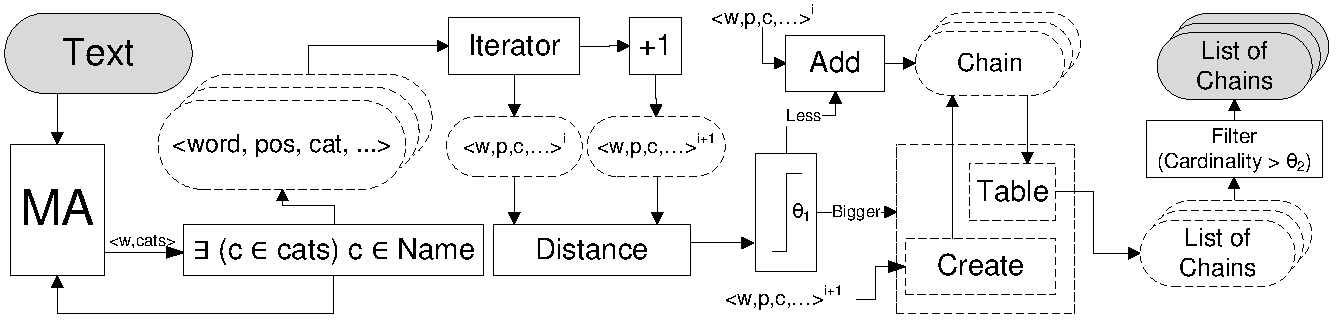
\includegraphics{figs/detailed_submachine.pdf}
%}
%\caption{The sequence of narrators extractor diagram}
%\label{f:sequence}
%}
%\end{figure*}

\novocalize

\transfalse
\begin{figure}[tb]
\center{
\resizebox{.95\columnwidth}{!}
{ \input{figs/exhadith2cols.pdftex_t}}
\caption{Hadith narrator sequence example.}
\label{f:exhadith}
}
\end{figure}
\transtrue
\vocalize

Several researchers~\cite{iTree,Hadithopaedia:08} attempted to automate 
the analysis of the hadith literature. 
We fully automate the analysis of three books of hadith selected 
arbitrarily~\cite{IbnHanbal,AlKulayni,AlTousi}~\footnote{We obtained
  the digitized books from 
  \href{http://www.yasoob.com/}{http://www.yasoob.com/} and 
  \href{http://www.al-eman.com/}{http://www.al-eman.com/}. }.
We accept a book as input
and segment it into a vector of hadiths,
and segment each hadith into its sanad and matn parts. 
We detect the sequence of narrators in the sanad and 
the relation that links each narrator to his ancestor and 
predecessor in the sequence. 
We also detect the full name of each narrator that is
composed of several proper names with connectors
in between. 

%NRC=19 descriptions= 91 stems
%family nmc connectors (all)=15 descriptions=33stems
%       ibn=1 descriptions=3 stems
%       2ab =2 descriptions=11 stems
%       2om=4 descriptions =5stems

To do that, we augmented our lexicon with person names obtained from online and Biblical sources,
and augmented the tag set of our lexicon with the following categories.
\begin{itemize}
\item $\mathit{NAME}$: a proper name of a person such as \RL{'a.hmad}. (2,500 male and 3,327 female lexicon items). 
\item $\mathit{IBN}$: a special name connector meaning ``the child of'' such as \RL{ibn}. (3 lexicon items expressing child,
11 expressing father, and 5 expressing mother relations).
\item $\mathit{NMC}$: name connectors that may be any word appearing amongst the other name connector categories. (33 lexicon items).
\item $\mathit{NISBA}$: a possessive adjective that qualifies a person such as \RL{alma.sriy} ``the Egyptian''. (4,698 possessive city or town, 82 country, and 4 continent items). 
\item $\mathit{NRC}$: a narrator connector such as
\RL{`an} ``on behalf of'', \RL{.hada_t} ``narrated'', \RL{qaal} ``said'', \RL{'a_hbar} ``told'' or one of their morphological equivalents. (91 lexicon items).
\end{itemize}
The categories can also be inferred from the concatenation of the tagged morphemes.

\subsection{The hadith finite state transducer}
\label{sec:FST}
% FSM for the FST

We implemented our hadith sequence extraction 
in an FST that reports a valid sequence
of narrators when a sequence of names
connected by narrator connectors appears. 
%This includes the task of finding multi-word names
%such as \RL{`bd alr.hmn} often appearing as ``run-on'' words.
The FST marks the beginning and the end of the hadith with 
the beginning of the current name sequence
and the beginning of the next name sequence, respectively.
%It detects the sequence of narrators as the sequence itself. 

%The FST also targets words that mean ``narrate'' when
%they appear between proper names. 
We illustrate the hadith FST
in Figure~\ref{f:hadith}(a). 
The transitions are  labeled with expressions
that operate on the category tags 
generated from the morphological analyzer.
The FST has four abstract states.
State $\mathit{TEXT\_S}$ is the initial state and denotes 
that the FST is outside the context of a sanad.
State $\mathit{NAME\_S}$ denotes that the FST is in
the middle of a sequence and has met a name. 
State $\mathit{NMC\_S}$ denotes that the FST is in
the middle of a narrator name.
State $\mathit{NRC\_S}$ denotes that the FST is 
in the context of a narrator name and the FST 
has met a narrator connector and is ready to meet 
a new narrator. 

The threshold $\theta_{\mathit{nmc}}$ 
corresponds to the number of tolerated name connectors 
that may occur between two names. %3
The symbol $\mathit{LIST}_{\mathit{nmc}}$ corresponds to the list 
of name connectors collected since the FST
started looping in the state $\mathit{NMC\_S}$.
The symbol $\lambda_{\mathit{nmc}}$ is a parameter 
that corresponds to a relaxed tolerance measure that
the FST resorts to in case the words separating
two names were longer than $\theta_{\mathit{nmc}}$ but 
contained a name connector word such as $\mathit{IBN}$ 
or $\mathit{NISBA}$.

The FST moves to state $\mathit{NAME\_S}$ on
$\mathit{NAME}$.
It moves to state $\mathit{NRC\_S}$ 
when Sarf reports an $\mathit{NRC}$.
State $\mathit{NMC\_S}$
indicates that the FST expects a name to appear within 
a tolerance threshold expressed by 
$\theta_{\mathit{nmc}}$ and $\lambda_{\mathit{bmc}}$.
It returns to $\mathit{NAME\_S}$ when a name is met, 
loops when still within the threshold, and 
resets to $\mathit{TEXT\_S}$ when the threshold is exceeded 
signaling that the last collection of names met do not qualify
as a narrator or a sequence of narrators. 

Similarly, $\mathit{NRC\_S}$ 
tolerates $\theta_{\mathit{nrc}}$ words 
before it gives up on its expectations. 
Note that we reach the $\mathit{NAME\_S}$
state only when a
valid $\mathit{NAME}$ is detected and we leave when no 
more $\mathit{NAME}$'s are detected.
The $\mathit{NRC\_S}$ state can only be reached if an 
$\mathit{NRC}$ is detected.
The state $\mathit{NMC\_S}$ can only be reached from a 
$\mathit{NAME\_S}$ state.

Whenever the FST transitions to $\mathit{NRC\_S}$ from either
$\mathit{NAME\_S}$ or $\mathit{NMC\_S}$, the FST reports 
a narrator detected and adds it to $\mathit{LIST}_{\mathit{narr}}$.
Whenever the FST transitions back to $\mathit{TEXT\_S}$,
the FST reports a sanad detected if 
$|\mathit{LIST}_{\mathit{narr}}| \ge N_{min}$ where 
$\mathit{LIST}_{\mathit{narr}}$ is the list 
of detected narrators and $N_{min}$ is a threshold denoting 
the minimum number of narrators required in a sanad.

We used the values of 3, 5 and 5 for $\theta_{\mathit{nmc}}$, 
$\lambda_{\mathit{nmc}}$, and 
$\theta_{\mathit{nrc}}$, respectively to obtain the results in 
Table~\ref{t:hadithresults}.

\begin{figure}[tb!]
\center{
\begin{tabular} {cc}
\resizebox{.45\columnwidth}{!}
{ \input{figs/hadith.pdftex_t}} 
&
\resizebox{.55\columnwidth}{!}
{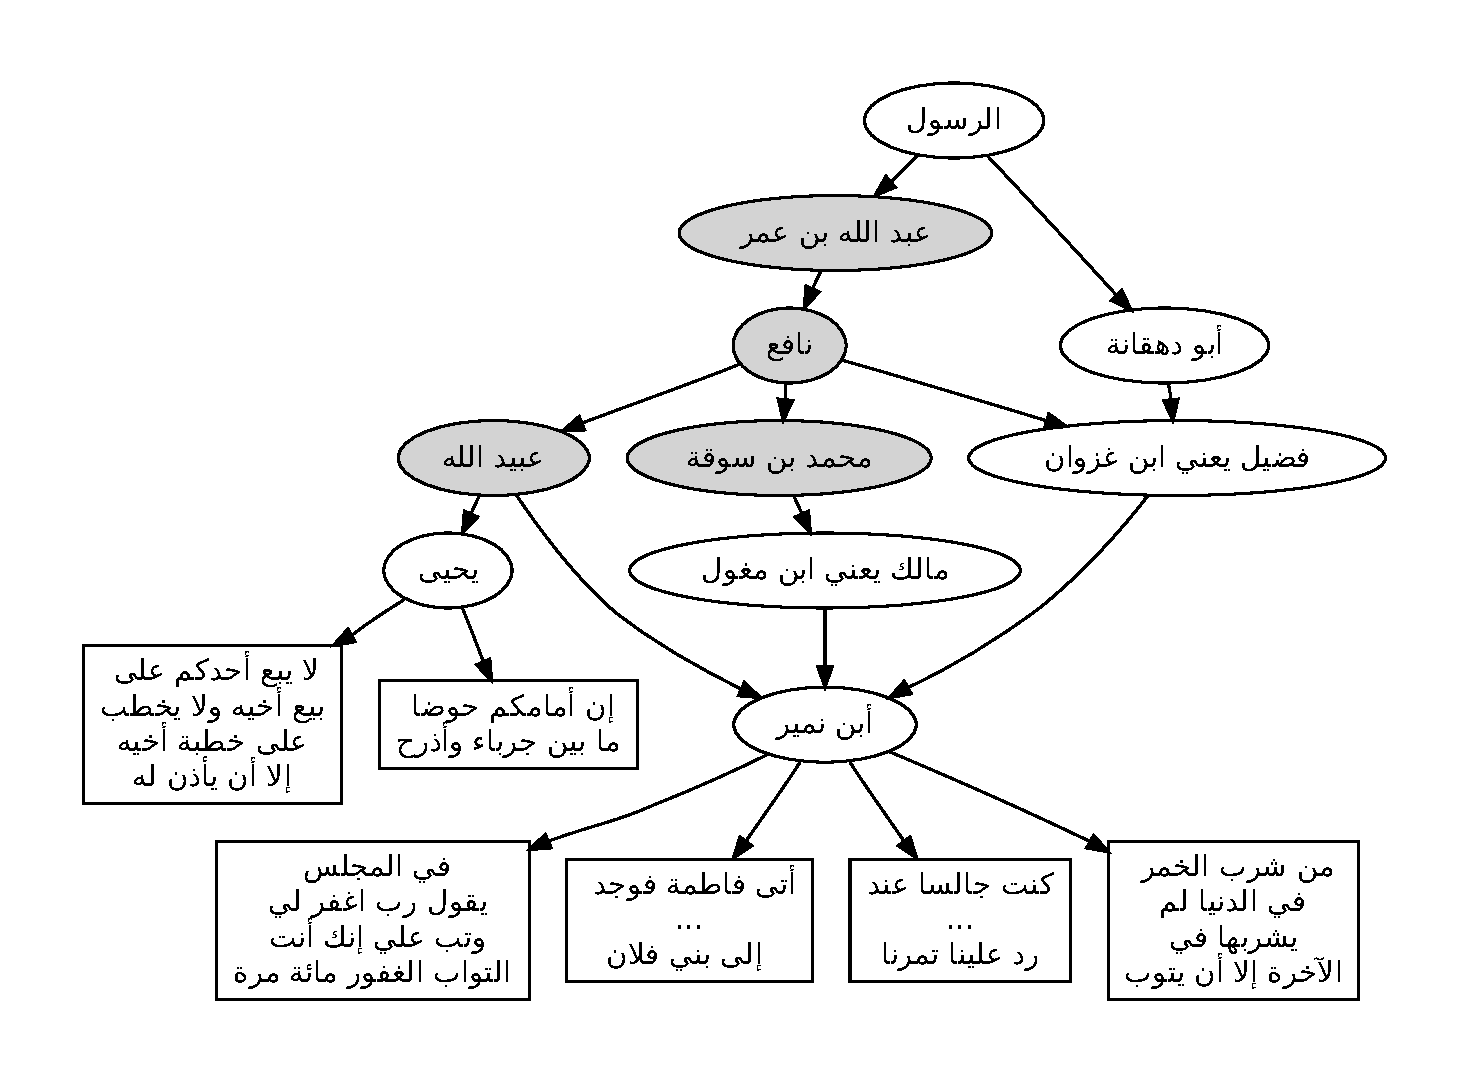
\includegraphics{figs/DAG_narrator.pdf}} \\
(a) FST & (b) Extracted narrator graph 
\end{tabular}
\caption{Hadith application.}
\label{f:hadith}
}
\end{figure}



%\begin{figure}[tb!]
%\center{
%\resizebox{.6\columnwidth}{!}
%{ \input{figs/hadith.pdftex_t}}
%\caption{The FST of the hadith application.}
%\label{f:hadith}
%}
%\end{figure}

%The definition of input labels such as NAME and IBN depends on the 
%morphological analyzer. 
%However, our case-based FST approach was able to perform well
%under both Sarf and a refined version of Sarf.

%\subsection{Optimizations}
%
%In addition to the FST, 
%NaGEMA uses punctuation marks to refine its analysis and 
%increase the accuracy of name detection, narration detection and narrator boundaries. 
%It also learns narrator names from simple patterns that 
%happen within narrator connectors and that are not 
%reported by Sarf as names. 
%NaGEMA learns names of narrators that consist of words missing from 
%the Sarf lexicon.
%NaGEMA learns the narrator names based on their context as they occurred 
%between narrator connectors or contained name connectors. 
%
%(explain better and merged information present about them in "Results" section)
%
\subsection{Extracting the narrator graph using node merge and split transformations}
\label{sec:graph}

%\begin{figure}[tb]
%\center{
%\resizebox{.8\columnwidth}{!}
%%{\includegraphics{figs/narrator_sequence_output.pdf}}
%{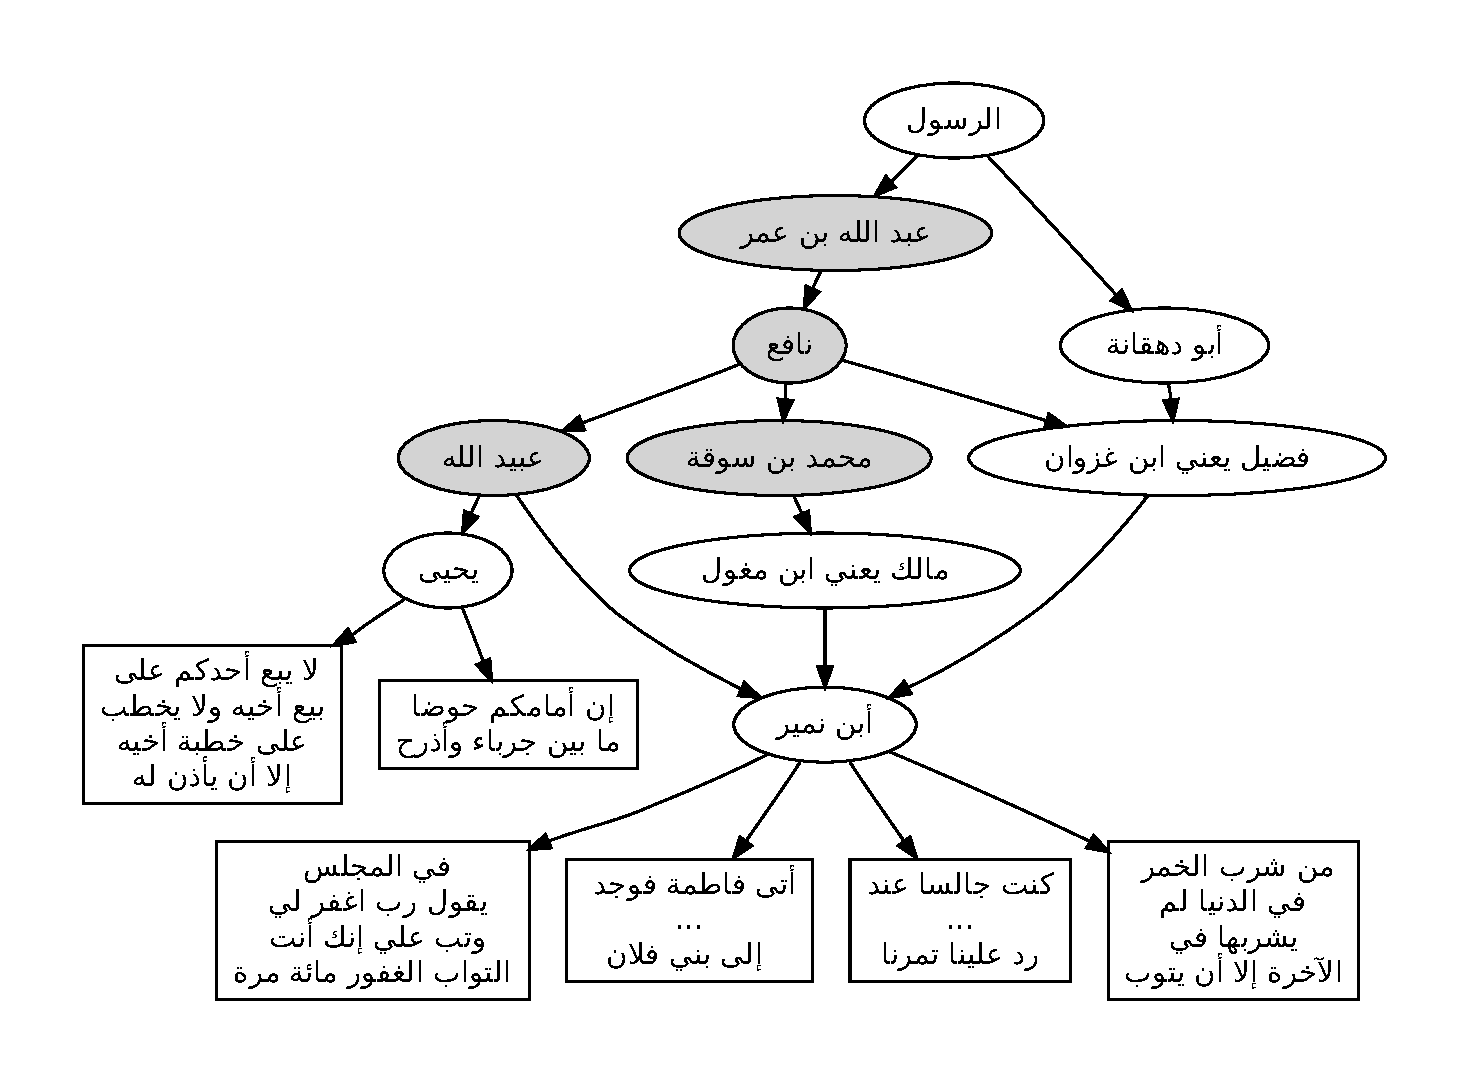
\includegraphics{figs/DAG_narrator.pdf}}
%\caption{Narrator directed acyclic graph 
%    extracted using NaGEMA }
%\label{f:narrators} 
%}
%\end{figure}

The hadith FST generates sequences of hadith narrators
such as $\langle n_1,n_2,n_3,n_4,n_5 \rangle$ shown in 
Figure~\ref{f:exhadith}. 
Our target is to automate the extraction of 
narrator graphs,
similar to the directed acyclic graph (DAG) 
in Figure~\ref{f:hadith}(b),
from one or more narration books
%We automatically extracted the POR from the three books of 
%hadith~\cite{IbnHanbal,AlKulayni,AlTousi}.
The nodes in boxes are the \RL{matn} of the hadith, 
and the other nodes are the narrators.

Our method uses two graph transformations to build the narrator
graph. 
It considers the graph with the disconnected sequence components, 
and performs a sequence of {\em merge} transformation 
for nodes that
represent equivalent narrators. 
A merge transformation takes two equivalent nodes $n_1$ and $n_2$,
appends the edge list of $n_2$ to that of $n_1$,
directs the incoming edges of $n_2$ to $n_1$,
and finally removes $n_2$ from the graph.
   
Then the method checks for cycles in the graph
introduced by the merge transformations and breaks the cycles
using node split transformations. 
The method also reports the cycles that require splitting nodes 
with high equivalency values to the user since such cycles may
indicate inconsistencies or fabricated narrations.

Scholars can use the narrator graph to perform interesting queries 
that were not possible before such as 
{\bf (1)} find important narrators who happen to be 
articulation nodes in the narrator graph,  and
{\bf (2)} conduct what-if analysis by simulating 
the effect of removing a narrator on the hadith literature
as several hadith with the same content 
may have several different narration sequences. 

%\subsection{Graph merge Algorithm}
%
%(modify according to hash)
%
%\begin{table}[tb]
%%\centering
%%\resizebox{.9\columnwidth}{!}{
%\begin{tabular} {p{6cm}}
%\begin{Verbatim}[fontsize=\relsize{-2},
%frame=topline,framesep=4mm,label=\fbox{Merge Algorithm},
%commandchars=\\\{\}, codes={\catcode`$=3\catcode`_=8}]
%Merge(sequence $C$[])
%  sequence $C_c$[]=\{\}
%  foreach sequence $c_1$ in $C$ 
%    $C_c = C_c \cup c_1$
%    foreach sequence $c_2$ in $C-C_c$
%      foreach Narrator $n_1$ in $c_1$
%        start = max( $n_1$.index - radius, 0)
%        end = min($n_1$.index + radius, $n_2$.size)
%        $n_2$ = $c_2$[start]
%        while (true)
%          if (Distance($n_1$, $n_2$) < $\theta$)
%            mergeNodes($n_1$, $n_2$)
%          if ($n_2$ = $c_2$[end])
%            break
%          $n_2$ = $c_2$.next($n_2$)        
%\end{Verbatim}
%\end{tabular}
%%}
%\label{t:merge}
%\end{table}
%

%The \CodeIn{Merge} Algorithm 
%iterates over the sequences of narrators looking 
%for equivalent narrators and merges the equivalent
%narrators.
%The \CodeIn{radius} parameter refines the search 
%to only consider narrators who belong to the same 
%generation. 
%For example, a narrator relating directly to the prophet
%is definitely not equivalent to a narrator separated
%from the prophet by ten or more narrators. 

%
%\begin{table}[tb]
%%\centering
%%\resizebox{.9\columnwidth}{!}{
%\begin{tabular} {p{6cm}}
%\begin{Verbatim}[fontsize=\relsize{-2},
%frame=topline,framesep=4mm,label=\fbox{Narrator distance metric },
%commandchars=\\\{\}, codes={\catcode`$=3\catcode`_=8}]
%Distance(Narrator n1, Narrator n2)
%  $N_1$ = stems(n1.names)
%  $N_2$ = stems(n2.names)
%
%  $E_n$ = getEqualNames($N_1$, $N_2$)
%  if ( $E_n$.isEmpty ) 
%      return $\infty$
%  if ( $E_n$.size $\ge$ min($N_1$.size,$N_2$.size))
%    dist -= $\delta_1$
%  if ($E_n$.equalNamesInOrder())  
%    dist -= $\delta_2$
%
%  $I_1$ = extractIbn( stems(n1.connectors) )
%  $I_2$ = extractIbn( stems(n2.connectors) )
%  $C_1$ = stems(n1.connectors - $I_1$)
%  $C_2$ = stems(n2.connectors - $I_2$)
%  if ($C_1 \cap$ Places $\not= C_2 \cap$ Places)
%    dist += $\delta_3$
%  else
%    dist -= $\delta_3$
%
%  $E_c$ = getEqualConnectors($C_1$, $C_2$)
%  dist -= $E_c$.size * $\delta_4$ 
%
%  if (correctIbnCorrespondence($I_1$, $I_2$))
%      dist -= $\delta_5$
%  return (MAX - dist)
%\end{Verbatim}
%\end{tabular}
%%}
%\end{table}

%\subsection{Narrator distance metric}
%MultiKey Hashing
%explain what are the keys used for each value and why suitable
% and say that we use the computed keys also conduct the 
% biography lookup
%Two narrator names may refer to the same person but may 
%differ in text and in structure. 
%For example, the names \noTrutfRL{عبد الله بن عمر}, 
%\noTrutfRL{ابن عمر}, and \noTrutfRL{ابن عمر رضي الله عنه}
%refer to the same person. 
%Our metric uses the \noTrutfRL{ابن} (son) name connector and 
%its morphological equivalents to order the person names
%that appear within a narrator entity. 
%The metric compares the name hierarchy and if the hierarchy 
%does not match, as in the case of 
%\noTrutfRL{عبيد الله بن عبد الله بن عمر}  and his parent 
%\noTrutfRL{عبد الله بن عمر},
%the metric returns \cci{false}.
%The metric also compares name qualifiers and if two name 
%qualifiers of the same morphological POS tag,  
%such as the place possessive qualifiers 
%\utfRL{العراقي} (the Iraqi) and \utfRL{المصري} (the Egyptian) 
%conflict, the metric returns \cci{false}.
%The metric then compares the morphological stems of the person 
%names that are in order, ignores the ones that are not in order,
%and computes the fraction of the matching names.
%
%Both our metric and the Levenshtein distance metric 
%used in~\cite{Azmi-2010}
%achieved 100\% precision on an arbitrarily selected set that 
%included 208 narrator pairs with 102 equal narrators.
%Our metric achieved 95\% recall versus 72\% recall for the 
%Levenshtein distance metric. 
%Which means that both metrics do not announce names equal if they
%are not, but our metric is better at detecting equal names.
%We believe that our metric is adequate to compare 
%complex Arabic names including contemporary ones in general.

%\section{The biography application}
%Biography books include one or more short biography 
%for each hadith narrator. 
%The short biography may contain information 
%about the dates and locations of birth and death, 
%the professors and the students of the narrator,
%and one or more evaluations of the credibility of the narrator. 
%
%We use a similar approach to the hadith application
%to locate narrator names within the biography books. 
%A biography text may contain the name of the narrator described
%in the biography as well as the names of other narrators who happen
%to be the professors, students, or the persons who evaluated the 
%narrator.
%Our method uses the narrator graph 
%extracted from several hadith books 
%as described earlier to segment the biographies
%and detect the owner of each biography. 
%
%Once our method detects a narrator, it colors the node in  the 
%narrator graph corresponding to it. 
%The professors and students of the narrator
%are the neighbors of the 
%node corresponding to the narrator in the graph. 
%Consequently, whenever a detected narrator entity 
%moves away from the 
%colored local cluster in the narrator graph, 
%we change the color and infer that we moved to a separate
%biography.
%The owner of each biography is the narrator at the center of the
%colored graph.
%
%The naive implementation of this approach is computationally
%expensive as it requires searching for each discovered narrator
%in the narrator graph. 
%We implemented a multi-hash narrator technique to 
%improve narrator localization in the graph and in the biography 
%books where we associate
%each narrator with all narrator names that can be generated 
%from its structure and compute a hash key and a relevance score 
%for that association. 
%We omit the discussion for brevity and we will report on that 
%elsewhere. 
%
%Scholars can use the located biographies to annotate
%each narrator with corresponding biographies thus automating
%the task of hadith authentication checks. 
%They can also annotate the narrator graph narrator graph with the locations and 
%the lifetime of the narrators and 
%check for time and location overlap that are necessary conditions
%for the consistency of two 
%neighboring narrators. 
%Scholars can also use the method to check the correspondence
%of different biography and hadith books. 
%
%We believe that this is the first work that applies
%{\em Arabic cross-document NLP}, and we believe
%that this approach can be extended to several applications
%such as the cross analysis of (1) investigation versus 
%interrogation reports, and (2) insurance claims versus 
%accident police reports to find inconsistencies. 

\section{Genealogical family tree application}

\begin{figure}
\center{
%\resizebox{0.9\columnwidth}{!}{
\tiny
\begin{tabular}{cp{.1cm}c}
\parbox[b]{.45\columnwidth}{
\utfRL{وَهذِهِ مَوَالِيدُ 
\emph{تَارَحَ}: وَلَدَ \emph{تَارَحُ} \emph{أَبْرَامَ} وَ \emph{نَاحُورَ} 
وَ \emph{هَارَانَ}. 
وَوَلَدَ \emph{هَارَانُ} \emph{لُوطًا}. 
وَمَاتَ \emph{هَارَانُ} قَبْلَ \emph{تَارَحَ} أَبِيهِ فِي أَرْضِ مِيلاَدِهِ فِي 
أُورِ الْكَلْدَانِيِّينَ. 
وَاتَّخَذَ \emph{أَبْرَامُ} وَ \emph{نَاحُورُ} لأَنْفُسِهِمَا امْرَأَتَيْنِ: 
اسْمُ امْرَأَةِ \emph{أَبْرَامَ} \emph{سَارَايُ}، 
وَاسْمُ امْرَأَةِ \emph{نَاحُورَ} \emph{مِلْكَةُ} بِنْتُ \emph{هَارَانَ}، 
أَبِي \emph{مِلْكَةَ} وَأَبِي \emph{يِسْكَةَ}}.

And the following are the heirs of Terah. 
Terah became the father of Abram, Nahor and Haran; and Haran became the father of Lot. Haran before died before the death of 
his father Terah in his mother land, in Ur of the Chaldeans. 
Abram and Nahor took wives for themselves: the name of Abram’s wife was Sarai; and the name of Nahor’s wife was Milcah, the daughter of Haran, the father of Milcah and Iscah.
}
& &
\resizebox{.55\columnwidth}{!}
{\includegraphics{figs/exgenesis.pdf}} \\
(a) Genesis 11:27-29 & & (b) Extracted family tree
\end{tabular}
\normalsize
\caption{Genealogy example.}
\label{f:genelists}
}
%}
\end{figure}

%In many cases, 
%there is an overlap between the many individual lists available across the Bible. When such an overlap occurs 
%meticulous readers can detect some seeming contradictions, in many cases due to conflicts or omissions.
%Detecting those conflicts is a task that has been performed by countless 
%number of Bible students, theologians and historians. 

%The importance of such lists was profound for the old nation of Israel. They 


%The genealogical lists established the kingship lineage and determined
%rights and privileges in the temple. Genealogical lists also determined descent with all its implications in biblical times
%such as the concept of reverted ownership of sold real estate; every fifty years ownership of sold land reverted to the 
%original owners and their inheritors. Genealogical lists were preserved due to the possible privilege of being the ancestor of the awaited Messiah.~\cite{catholicEncyclopedia:Online}
%
%For many believers, genealogies are used as the main indicators of chronology especially when calculating the age of mankind~\cite{Thomas:92}.
%Believers used them to defend the historicity of Biblical events and characters against other accounts from other 
%texts thought of as fables and myths. 
Biblical genealogical lists 
trace key biblical figures such as 
Israelite kings and prophets.
The example in 
Figure~\ref{f:genelists}(a)
from Genesis that traces the
heirs of \utfRL{تارح} (Terah).
%They contain person names
%and kinship relations between the names. 
Separate genealogical lists that overlap may have consistency 
%issues~\cite{catholicEncyclopedia:Online,Belote:Online,completeBibleGenealogy:Online}. 
issues~\cite{completeBibleGenealogy:Online}. 
For example, Matthew and Luke report two different 
genealogies of Jesus. 
Scholars constructed partial genealogical graphs 
manually from several lists
and their work is short from being 
comprehensive~\cite{Belote:Online,SoulLiberty:Online}.
Creating a comprehensive genealogical graph from all biblical 
accounts greatly enhances the study of the bible. 
Such comprehensive graphs can be tagged
with time durations between a parent and the birth of 
its children as is common in many biblical accounts. 

Our method takes as input Arabic text with a genealogical
list such as the genealogical list in
Figure~\ref{f:genelists}(a) 
and automatically extracts the genealogical family tree 
where person names are entities and edges represent 
``spouse'' and ``child'' labels such as 
Figure~\ref{f:genelists}(b).
We marked the person names with bars above them, and we 
filled the spouse nodes with grey. 
To perform this task, our method first passes the text to
Sarf, the morphological analyzer, that reports detected morphemes 
with their corresponding tags. 

We augmented the tag set of Sarf with 
the following categories relevant to the genealogical 
application. 
\begin{itemize}
\item {\em NAME} a person name that can be either male or female. 509 lexicon items. 
\item {\em CHILD} a connector with a descent semantics such as \utfRL{ابن} (son). 12 lexicon items. 
\item {\em CHILDREN} a connector with a plural descent semantics such as \utfRL{ابناء} (children). 16 lexicon items. 
\item {\em PARENT} a connector with parenthood semantics such as \utfRL{أباه} (his father). 7 lexicon items. 
\item {\em SPOUSE} a connector with marital partnership semantics such as \utfRL{سريّته} (his concubine). 11 lexicon items. 
\item {\em SPOUSES} a connector with plural partnership semantics such as \utfRL{سراري} (his concubines). 7 lexicon items. 
\item {\em SIBLING} a connector with sisterhood semantics such as \utfRL{أخيه} (his brother). 14 lexicon items.
\item {\em SIBLINGS} a connector with plural sisterhood semantics such as \utfRL{اخوته} (his siblings). 18 lexicon items. 
\end{itemize}
Note that (1) some lexicon items might be categorized into 
more than one of the above categories, and 
(2) the method infers the gender from POS and gloss tags 
of the person name as well as from those of the 
other categories. 
In case of conflict, the method gives precedence to the 
gender inferred from the person names. 
Note also that the phrases
\utfRL{اسحاق بن يعقوب} (Izhac - son of - Jacob)
and 
\utfRL{اسحاق ابنه يعقوب} (Izhac - his son - Jacob)
contain the same named entities, and are identical 
as far as stemming is concerned. 
However, the analysis 
of the suffix morphemes of \utfRL{ابنه} results in inferring
a parent category in the second phrase.

The method considers the detected categories and passes 
them to a genealogy FST.
The genealogy FST distinguishes detected names as follows. 
\begin{itemize}
\item {\em NAME} denotes a newly detected name that is not 
a node in the current tree. 
\item {\em LEAF} denotes a name that is a leaf in the current tree.
\item {\em NODE} denotes a name that is an internal node in the current tree.
\end{itemize}
The rest of the categories are presented to the FST as is and
are all denoted with {\em EDGE}. 

\begin{table}[bt]
\centering
\caption{State transitions and actions for genealogy application.}
\begin{tabular}{cp{.1cm}p{1.1in}cp{2.4in}}
State & & Input & Transition & Actions and output \\ \hline
\multirow{3}{*}{\em Text} 
&  & $n=\mbox{NAME}$                   & {\em Parent} & addNode(n), $n_i = n, w = 0, e_i=\mbox{CHILD}$ \\ \cline{3-5}
&  & $n=\mbox{LEAF} \vee \mbox{NODE}$ & {\em Parent} & $n_i = n, w = 0, e_i=\mbox{CHILD}$ \\ \cline{3-5}
&  & $e=\mbox{EDGE}$                   & {\em Parent} & $n_i = \empty, w = 0, e_i=e$ \\ \hline
\multirow{5}{*}{\em Parent} 
&  & $n=\mbox{NAME}$                   & {\em Parent} & addNode($n$), addEdge($n_i$,$n$,$e_i$), $n_i = n, w = 0$ \\ \cline{3-5}
&  & $n=\mbox{LEAF}$                   & {\em Child}  & $n_i = n$ \\ \cline{3-5}
&  & $e=\mbox{EDGE}$                   & {\em Parent} & $w = 0, e_i=e$ \\ \cline{3-5}
&  & otherwise $\wedge w \le \theta$   & {\em Parent} & $w=w+1$, add unclassified edges and nodes \\ \cline{3-5}
&  & otherwise $\wedge w > \theta$     & {\em Text}   & local tree detected \\ \hline
\multirow{5}{*}{\em Child} 
&  & $n=\mbox{NAME}$                   & {\em Child}  & addNode($n$), addEdge($n_i$,$n$,$e_i$) \\ \cline{3-5}
&  & $n=\mbox{LEAF}$                   & {\em Child}  & $n_i = n$ \\ \cline{3-5}
&  & $e=\mbox{EDGE}$                   & {\em Parent} & $w = 0, e_i=e$ \\ \cline{3-5}
&  & $\mbox{ENDLINE}$                  & {\em Parent} & $w = 0$ \\ \cline{3-5}
&  & otherwise                         & {\em Child}  & add unclassified edges and nodes \\ \hline
\end{tabular}
\label{t:genefst}
\end{table}

Table~\ref{t:genefst} described the states, input, transitions and the actions and outputs of the genealogy FST. 
The FST keeps track of the last detected {\em NODE} and {\em EDGE} in the state elements $n_i$ and $e_i$.
It also keeps track of the number of the words in sequence that do not match a category in $w$. 
Once $w$ passes the threshold $\theta$, and if the FST has any nodes and edges detected, the tree is reported as output. 
The FST has three abstract states where {\em Text} 
is the initial state and denotes that the FST is outside the context of a genealogical list.
State {\em Parent} denotes that the FST is in the middle of a genealogical list and has met some names. 
State {\em Child} denotes that the FST is in the middle of a genealogical list and in the context of names of children of a discovered 
name. 
When a {\em NAME} is met, the FST adds a node and possibly and edge to the tree. 
When a {\em NODE} or a {\em LEAF} is met, the FST adds
an edge to the tree. 
When words that do not belong to the specified categories are met between {\em EDGE} words or 
between {\em NAME, LEAF}, or {\em NODE} words the FST adds them as labels to unclassified edges. 
The FST uses these unclassified names and edges to learn edge 
semantics that can help in a subsequent run to resolve 
ambiguities; connected nodes with un-classified edges. 

The FST produces a set of genealogical trees. The method takes those trees and merges equivalent 
nodes to build a global genealogical tree. 
The method merges nodes with the same names and whose merger does not cause a cycle in the genealogical tree with only the 
``child'' and ``spouse'' edges considered. 

\section{Related work }
\label{s:related}

%\transfalse
%\novocalize
%\begin{figure*}[tb]
%\center{
%\resizebox{1.8\columnwidth}{!}
%%{ \input{iTreeMohamada}}
%{\includegraphics{iTreeMohamada}}
%\caption{Output of iTree fails to detect \RL{m_hmdA}.}
%\label{f:mohamada}
%}
%\end{figure*}
%\transtrue

The  iTree~\cite{Azmi-2010,iTree} tool
uses a context free grammar (CFG) approach to solve 
the narrator extraction problem. 
It preprocesses the text to remove punctuation and diacritics 
and to normalize white spaces, and uses a similarity-based approach
to memory based learning~\cite{Azmi-2010} 
in order to perform shallow parsing of the preprocessed text. 
The iTree CFG enumerates several stop phrases that surround
names narrators.
The iTree tool fails when a morphological variation of 
one of the stop phrases occurs.
%For example, Figure~\ref{f:mohamada} extracted 
%using iTree fails to detect \RL{m_hmdA} as a name of the
%prophet and does not stop at it when computing the sequence 
%of the hadith
%\transfalse
%\setcode{utf8}
%%\begin{arabtext}
%\RL{
%حدثنا وكيع، حدثني سعيد بن السائب، عن داود بن أبي عاصم الثقفي، قال
%سألت ابن عمر عن الصلاة، بمنى فقال هل سمعت {\bf محمدا}، صلى الله عليه وسلم قلت
%نعم وآمنت فاهتديت به قال فإنه كان يصلي بمنى ركعتين.
%%\end{arabtext}
%}
%\setcode{standard}
%\transtrue
%\vocalize
We differ in that we do not preprocess the text,
we use morphological analysis,
and we do not base our method
on stop phrases that surround narrator names. 
Rather, we assume that narrator names are likely to happen in 
localities with a high number of person names. 
We use narrator connectors and their
morphological equivalents and thus we do not suffer from 
the ``parser noise words'' problem of iTree. 
The iTree tool extracts successfully 86.7\% of
the narration sequences of 90 selected traditions with 
34 simple cases and 56 hard cases. 
We ran our method against the five hadith that ship with
iTree and the two hadith from the iTree
paper and we were able to extract all narration
sequences even on the examples where iTree
reports a ``parser noise'' problem.

%As we do not have access to the selected
%90 traditions iTree reports on, we claim
%that NaGEMA outperforms iTree as it works on
%the full text of the presented hadith books
%and reports a higher success rate. 

Our NE detection method differs from 
local grammar based approaches~\cite{ZAGHOUANI10,Traboulsi:09}
in that they enumerate several local grammar rules
to capture the desired named entities, 
and use techniques to automatically compute finite state 
machines that detect the structures expressed in the 
local grammars.
The work in~\cite{ZAGHOUANI10} uses morphological stemming
for Arabic with local grammars developed for Latin languages 
and suited to fit Arabic and reports 87\% precision and 
66\% recall for person names. 
Similarly, the work in~\cite{jumaily2011,TAGARAB98} 
uses morphological stemming and pattern matching. 
We differ in that we are not limited to the use of stems 
and we use the augmented
set of morphological tags for all prefixes and suffixes as well.
This allows us to lift the restriction of the stop words 
used in local grammars and in~\cite{Abuleil04}.
We also differ in that we directly build the
FST to detect the named entities as well 
as the relational entities, 
we do not enumerate all the structures that express our targeted
entities, and we are not restricted to the expressive power of 
a local grammar language where it is often not intuitive 
(and in cases not possible) to express thresholds using regular 
expressions. 
In the future, we plan to develop a local
grammar language that has that expressive power.

ANERSys boosts its capabilities to detect named entities by using 
task specific corpora and gazetteers and ignores 
POS tags~\cite{Benajiba:07,Benajiba:08}. 
We are similar to ANERSys in that we augment the lexicon Sarf
with application relevant lexicon items and tags. 
We differ in that they use statistical analysis models such as
n-gram and maximum entropy measures.
In other work, they
achieve major improvements when they use lexical and
morphosyntactic features and a parallel Arabic and English 
corpora to bootstrap noisy features~\cite{BenajibaZDR10}. 

We differ from rule-based systems with local 
grammars~\cite{ShaalanR09} in that we our system 
uses FSTs instead of rules, and in that it can learn named 
entities and infer semantics
for entities that are equivalent within one or two graph 
transformations to predefined graph edge labels. 


\section{Results}
\label{sec:results}

%\begin{table}[bt]
%\centering
%\caption{Results of the hadith case study with Sarf.}
%%\begin{tabular}{|p{1.5cm}||c|c||c|c||c|c|} \hline
%\resizebox{1.1\columnwidth}{!}{
%\begin{tabular}{lcp{.2cm}cp{.2cm}c} %\cline{2-10}
% &  AlKafi & & AlIstibsar & &IbnHanbal \\ \cline{1-6}
%Word count  &98,943 & & 103,835 & & 20,354 \\ 
% Names       & 12,060  & & 14,613& & 3,013\\
%%Names/Narrator & 1.97 & & 1.84& & 1.25 \\
%Narrators  & 2,623 & & 5,767& & 1,755 \\ 
%%Narrators/sequence  & 4.84 & & 4.76 & &4.05 \\
%sequences  & 542 &  & 1,211& & 433 \\ 
%Ignored names  & 6,400 &  & 3,348 & & 642 \\ \hline
%Segmentation accuracy  & 96\%& & 96\%& & 92\%\\ 
%sequence accuracy & 99\%&  & 99\%& & 97\% \\ 
%%Narrator accuracy  & & & & &  & & & \\ 
%Narrator accuracy  & 91\%& & 90\% & & 90\% \\ \hline
%%Name false positives  & 7\%&  & 4\% & & 4\% \\ \hline
%Running time (secs.)& 1.32 & & 1.31 & & .096\\ \hline 
%\end{tabular}
%}
%\normalsize
%\label{t:hadithresallresults}
%\end{table}
%
%
%\begin{table*}[bt]                                     
%\centering                                            
%\caption{Hadith results compared with iTree. }
%\resizebox{.95\columnwidth}{!}{
%\begin{tabular}{p{2.1cm}lp{.1cm}cccp{.1cm}cccp{.1cm}ccc}
%%\multicolumn{13}{c}{NaGEMA with all refinements} \\ \cline{3-13}
%& & & \multicolumn{3}{c}{segmentation} & &  \multicolumn{3}{c}{sanad boundary}  & &  \multicolumn{3}{c}{name boundary} \\
%& & & recall & precision & F-score & & recall & precision & F-score & & recall & precision & F-score \\ \cline{2-14}
%\multirow{3}{*}{NaGEMA }&musnad & & 0.999 & 0.999 & 0.999 & & 0.993 & 0.990 & 0.991 & & 0.999 & 0.998 & 0.999 \\
%&kafi & & 0.999 & 0.920 & 0.958 & & 0.937 & 0.970 & 0.953 & & 0.993 & 0.988 & 0.990 \\
%&istibsar & & 0.999 & 0.973 & 0.986 & & 0.980 & 0.950 & 0.965 & & 0.996 & 0.998 & 0.997 \\ \cline{2-14}
%& & & 0.999 & 0.964 & 0.982 & & 0.970 & 0.970 & 0.970 & & 0.996 & 0.995 & 0.995 \\ \hline \hline
%%& & &  &  &  & &  &  &  & &  &  & \\
%%&\multicolumn{13}{c}{iTree} \\ \cline{3-13}
%& & & \multicolumn{3}{c}{accept as hadith} & &  \multicolumn{3}{c}{sanad boundary}  & &  \multicolumn{3}{c}{name boundary} \\
%& & & recall & precision & F-score & & recall & precision & F-score & & recall & precision & F-score \\ \cline{2-14}
%\multirow{3}{*}{iTree} &musnad & & 0.999 & NA & 0.999 & & 0.997 & 0.977 & 0.987 & & 0.998 & 0.999 & 0.999  \\
%&kafi & & 0.043 & NA & 0.083 & & 0.999 & 0.313 & 0.476 & & 0.999 & 0.999 & 0.999 \\
%&istibsar & & 0.028 & NA & 0.054 & & 0.875 & 0.583 & 0.700 & & 0.999 & 0.999 & 0.999 \\ \cline{2-14}
%& & & 0.357 & NA & 0.379 & & 0.957 & 0.624 & 0.721 & & 0.999 & 0.999 & 0.999 \\ 
% \end{tabular}                 
%}                             
%\normalsize                   
%\label{t:hadithresults} 
%\end{table*}                   

%\input{cicling/tables.tex}

We evaluated our method against three books of 
hadith~\cite{IbnHanbal,AlTousi,AlKulayni},
and the book of Genesis~\cite{}.
%and one book of biographies with several volumes~\cite{khoei}. 
We define our metrics, present our evaluation reference with interannotation agreement results, 
and then present the results for the hadith
and genealogical list applications.

{\bf Metrics.}~~
Segmentation recall refers to the ratio of the narrations correctly detected against the
total number of narrations present. 
Segmentation precision refers to the fraction of correctly detected narration sequences compared to all the extracted
narration sequences. 
Similarly, sanad boundary recall measures whether we detected all narrators
in the sanad; while sanad boundary precision measures whether we did so without introducing false positives. 
The same concept applies to the narrator boundary where we count the number of words constituting 
a valid narrator.
For the genealogy application, segmentation refers to the ratio of the genealogical lists correctly detected against the total 
number of lists present.
Segmentation precision refers to the fraction of correctly detected genealogical lists compared to all the extracted lists. 
Recall for genealogical boundary detection measures whether we detected all person names in the lists; 
precision measures whether we did so without introducing false positives.


{\bf Interannotation.}~~
We developed a GUI tool and asked two volunteers to tag the sanad boundaries and the narrator names therein for 10\% of the hadith text, 
and to tag the lists, the person names therein, and to edit the tree structure within the genealogy list for the Genesis.
%We computed the interannotation agreement metrics presented in Table~\ref{t:interannotator}.
The annotators agreed with above 98\% precision and recall on hadith segmentation, sanad boundaries and name boundaries.
The annotators agreed with 99\% and 97\% recall on genealogy segmentation and list boundaries.
They also scored 95\% precision on list boundaries.
For the genealogy segmentation, the tags of the first annotator were a subset of the tags of the second and therefore they scored  
39\% precision as we measured the second against the first.
The Genesis contains texts that are intended to describe genealogy, 
and also contains person names with mentions of family relations that are not intended to be genealogical lists.
The second annotator aggressively selected both types of genealogical lists, while the first annotator selected the first type and was 
very conservative in selecting the second type. 
Some genealogy lists may contain more than one family tree and our GUI was limited to allow the annotators to select one of the trees.
This resulted in a 65\% precision score for genealogy list boundaries agreement. 
The two annotators agreed on a reference tag set that we used to compute the following accuracy results. 


%
%\begin{table*}[bt]                                     
%\centering                                            
%\caption{Interannotator Agreement }
%\resizebox{1\columnwidth}{!}{
%\begin{tabular}{p{1.3cm}p{.1cm}cccp{.1cm}cccp{.1cm}ccc}
%%\multirow{2}{*}{Test Case} 
%& &  \multicolumn{3}{c}{segmentation} & &  \multicolumn{3}{c}{sanad/genealogy boundary}  & &  \multicolumn{3}{c}{name boundary} \\
% & &  recall & precision & average & & recall & precision & average & & recall & precision & average \\ \cline{3-5} \cline{7-9} \cline{11-13}
%Hadith &  & 0.976 & 0.999 & 0.988 & & 0.991 & 0.971 & 0.981 & & 0.999 & 0.997 & 0.998 \\ 
%Genealogy &  &  0.999 & 0.390 & 0.695 & & 0.969 & 0.954 & 0.812 & & NA & NA & NA\\
% \end{tabular}                 
%}                             
%\normalsize                   
%\label{t:interannotator} 
%\end{table*}    

{\bf Hadith application results.}~~
The results in Table~\ref{t:hadithresults} compare the results of our method against iTree~\cite{iTree} for the hadith application.
We augmented iTree with the list of names used by our method to conduct a fair assessment.
The iTree tool does not tackle the problem of segmentation as it
takes as input an isolated hadith. 
%In many cases iTree fails to recognize the structure of
%the hadith and does not extract any useful information from the narration. 
%This happens for example when a slight variation of the iTree grammar rules 
%happens first in the hadith.
In Table~\ref{t:hadithresults}, instead of the segmentation columns 
we report the percentage of times iTree succeeded to recognize the valid hadith we pass.
This measure is equivalent to recall; nonetheless, precision in this context is not applicable.

On average, our method acheived a 97\% segmentation recall rate compared to 35.7\% for iTree.
The difference depended highly on the book under consideration. 
For Musnad, both methods performed well;
however iTree reported less than 5\% recall for the Kafi and Istibsar books due
to the less structured nature of the narrations in both books.
%For example, iTree's grammar is defined such that a hadith starts by 
%an Ikhbar word (\noVocRL{AdaT al-A_hbAar}) such as
%\noVocRL{qAl} ``said'', \noVocRL{.hadda_t} ``narrated'', etc...; 
%however, the Kafi and Istibsar books followed a flexible style to express the narration 
For example, in a significant number of narrations a narrator name preceded narration words 
(\noVocRL{qAl} ``said'', \noVocRL{.hadda_t} ``narrated'', etc...) contrary to what iTree expects.
Note that it is not trivial (if even possible) to take care of this variation using local grammars 
and CFGs as this introduces a high level of ambiguity.
For the hadith that iTree succeeded to recognize, iTree had a lower sanad boundary precision (62.4\% on the average).
This is mainly due to the stop phrases used to detect the termination of sanad boundaries.
Sanad termination is often implicit in Kafi and Istibsar causing iTree to extend the boundary of the sanad until the next stop phrase.
Our method detects the end of the sanad when it meets a sequence of words of length $> \theta$ with no names.
The narrator boundary accuracy showed similar results between iTree and 
our method since we augmented iTree with the names from the lexicon of Sarf. 

\begin{table*}[bt]                                     
\centering                                            
\caption{Hadith results compared with iTree.}
\resizebox{1\columnwidth}{!}{
\begin{tabular}{lp{.1cm}cp{.1cm}cccp{.1cm}cccp{.1cm}ccc}
%\multicolumn{13}{c}{NaGEMA with all refinements} \\ \cline{3-13}
{\bf our} & & hadith & & \multicolumn{3}{c}{segmentation} & &  \multicolumn{3}{c}{sanad boundary}  & &  \multicolumn{3}{c}{narrator name boundary} \\
{\bf method} & & count & & recall & precision & F-score & & recall & precision & F-score & & recall & precision & F-score \\ 
    \cline{1-3} \cline{5-7} \cline{9-11} \cline{13-15}
musnad & & 212 & & 0.991 & 0.976 & 0.983 & & 0.969 & 0.967 & 0.968 & & 0.999 & 0.996 & 0.998 \\
kafi & & 199 & & 0.970 & 0.909 & 0.938 & & 0.934 & 0.954 & 0.944 & & 0.999 & 0.998 & 0.998 \\
istibsar  & & 189 & & 0.968 & 0.973 & 0.971 & & 0.946 & 0.945 & 0.945 & & 0.999 & 0.998 & 0.999 \\ \hline 
 & & 600 & & 0.976 & 0.953 & 0.964 & & 0.950 & 0.956 & 0.953 & & 0.999 & 0.997 & 0.998 \\ 
% \hline \\ \hline
 \\
%& & &  &  &  & &  &  &  & &  &  & \\
%&\multicolumn{13}{c}{iTree} \\ \cline{3-13}
{\bf iTree} & & hadith& & \multicolumn{3}{c}{accept as hadith}& & \multicolumn{3}{c}{sanad boundary} & & \multicolumn{3}{c}{narrator name boundary} \\
 & & count & & recall & precision & F-score & & recall & precision & F-score & & recall & precision & F-score \\ 
    \cline{1-3} \cline{5-7} \cline{9-11} \cline{13-15}
musnad && 62 && 0.999 & NA & NA & & 0.997 & 0.977 & 0.987 & & 0.998 & 0.999 & 0.999  \\
kafi && 23 && 0.043 & NA & NA & & 0.999 & 0.313 & 0.476 & & 0.999 & 0.999 & 0.999 \\
istibsar && 36 && 0.028 & NA & NA & & 0.875 & 0.583 & 0.700 & & 0.999 & 0.999 & 0.999 \\ \hline
 & & 124 && 0.357 & NA & NA & & 0.957 & 0.624 & 0.721 & & 0.999 & 0.999 & 0.999 \\ 
 \end{tabular}                 
}                          
\normalsize                   
\label{t:hadithresults} 
\end{table*}    

{\bf Narrator graph.}~~
The results in Table~\ref{t:PORnLearning}(a) report the precision and recall metrics for generating 
the full narrator graph via merging the detected hadith sequences.
For each narrator node, we computed the number of nodes it correctly merges with against the number of nodes it should merge with and 
averaged that across all nodes to compute the recall metric.
The precision metric denotes the average of the
ratio of correctly merged nodes against the number of merged 
nodes for each narrator node.

The ``detected'' row includes only the narrator nodes detected by our method and indicates the accuracy of the graph building routine 
isolated from the rest of the method.
The ``all'' row includes all narrators and sanads in the text.
The recall rate was 63\% mainly due to the conservative cycle breaking transformation that splits merged narrator nodes even if 
they were equivalent. 
We expected higher precision values than 82\% and 77\% and upon examining the results, we discovered two main issues. 
The first issue is in the reference graph since the manual annotator decided to keep nodes split whenever he was faced with
confusing cases such as the narrator nodes \utfRL{سعيد بن السائب}, \noTrutfRL{سعيد}, and \utfRL{سعيد بن جبير}. 
The text included several of these examples such as \utfRL{سليمان التيمي}, \utfRL{سليمان بن رزين}, and \utfRL{ سليمان بن موسى}.
The automated merging will make a decision to merge two of the three names in each case 
and uses other helper information such as the rank of the nodes in the graph to make a decision. 

The second issue has to do with the degree of equality checks that the merging algorithm performs when deciding to merge narrator nodes.
Consider three narrator nodes merged into one node $n_{merged}$.
Now consider merging a new narrator node $n_*$ with $n_{merged}$. 
We currently compare $n_*$ with only one of the constituents of 
$n_{merged}$ and make the simplifying assumption that our equality
metric is transitive. 
Comparing to more narrators in $n_{merged}$ helps improve precision. 


%In the POR, we have 2 ways of computing the accuracy, just as it is (all narrators), second (accounting for missing narrators in the trees in the first place which will result in having the errors of parsing accumulate over the merging of nodes (so in the detected narrators we calculate the results without expecting to find the undetected nodes (i.e. in recall we dont count nodes that are missing due to not having them in the first place)

 %           In all cases, there will still be accumulated errors in the POR due to errors in parsing, for example (boundaries of detected narrators will hurt accuracy) also if we have missing narrators or extra narrators in our POR we might get extra cycles and thus have to break nodes that should not be breaked. so in all cases, POR results have accumulated errors. But still the detected narrators measure is fairer.

\begin{table*}[bt]                                     
\centering                                            
\caption{Narrator graph and name learning results.}
\resizebox{1\columnwidth}{!}{
\begin{tabular}{cp{1cm}c}
	\begin{tabular}{p{1.5cm}p{.1cm}ccc}
    narrators & & recall & precision & F-score \\ \cline{1-1} \cline{3-5}
	detected  & & 0.673 & 0.824 & 0.741\\
	all       & &  0.632 & 0.771 & 0.694\\
	\multicolumn{5}{c}{(a) Narrator graph accuracy} \\
	\end{tabular}  
&  &
	\begin{tabular}{p{1.5cm}p{.1cm}ccc}
     names    & & recall & precision & F-score \\ \cline{1-1} \cline{3-5}
	 sanad    & &  0.649 & 0.940 & 0.768\\
	 all      & & 0.794 & 0.733 & 0.762\\
	\multicolumn{5}{c}{(b) Name learning accuracy} \\
	\end{tabular}  \\
 \end{tabular}               
}                             
\normalsize                   
\label{t:PORnLearning} 
\end{table*} 

{\bf Learning names.}~~
Table~\ref{t:PORnLearning}(b) reports the precision and recall of the names that our method learned from the 
books of hadith. 
Within the sanad segments, our method learned 65\% of the names it should learn with 94\% accuracy.
It learned 79\% of the names it should learn from the whole text at a 73\% precision. 
The precision is higher within the sanad since names are more frequent in the sanad context.
The recall is higher for the whole text since inside the sanad our method is more likely to resolve ambiguous tags 
as name and narrator connectors than if outside the sanad.

%
%{\bf Biography narrator detection.}~~
%Table~\ref{t:narratorDifference} shows the accuracy results for the narrator detection and the biography boundary detection
%for the Khoei biography book.
%The first row shows the results computed by considering the biography book alone without the help of the narrator graph
%extracted from the hadith books. 
%Without the narrator graph, our method detected 94\% of the narrators mentioned in the book with 81\% precision. 
%The method without the narrator graph, detected correctly (94\% precision) the boundaries of the biographies. 
%
%With the help of the narrator graph, our method detected 65\% of the narrator names in the biography book. 
%The rest of the names were simply not found in the hadith books that we used to generate the narrator graph. 
%With the use of the narrator graph and the coloring algorithm, our method detected the boundaries of the biographies
%with 93\% precision. 
%We believe that an exhaustive graph that includes narrator names from more books of hadith will improve the 65\% narrator 
%detection recall metric.
%In all cases, narrator names that exist in the biography and not in the hadith books are not of interest to the narrator
%graph annotation problem.
%
%%The numbers in the right hand side of Table~\ref{t:narratorDifference}  may explain why 
%Narrator detection in biography books is harder than in hadith books. 
%For example, the ratio of narrator names to the rest of the text is 22\% in Musnad while it is 49\% in Khoei,
%and the average length of a narrator sequence in Musnad is 2.6 narrators while it is 3.5 narrators in Khoei.
%With the use of the narrator graph extracted from the hadith books, our method was able to improve biography boundary detection
%from 41\% to 93\%.
%This is evidence that cross-document entity detection helps to accurately find named entities in harder NLP tasks. 
%
%\begin{table*}[bt]                                     
%\centering                                            
%\caption{Accuracy results for the biography application.}
%\resizebox{.7\columnwidth}{!}{
%
%%\begin{tabular}{cp{0.3cm}c}
%
%	\begin{tabular}{cp{.1cm}cccp{.1cm}ccc}
%	          & & \multicolumn{3}{c}{narrator detection} & &  \multicolumn{3}{c}{biography boundary} \\
%	 & & recall & precision & F-score & & recall & precision & F-score \\ 
% \cline{3-5} \cline{7-9}
%%hadith	 & sanad & & 0.923 & 0.999 & 0.960 & & 0.996 & 0.999 & 0.998  \\
%%(musnad) & all & & 0.954 & 0.961 & 0.958 & & 0.996 & 0.987 & 0.992 \\ 
%%	\hline \hline
%w/o graph & & 0.943 & 0.812 & 0.873 & & 0.407 & 0.945 & 0.569 \\
%with graph & & 0.654 & 0.909 & 0.760 & & 0.933 & 0.960 & 0.946 \\ % found in narrator graph
%	 \end{tabular}   
%%&  &
%%	\begin{tabular}{ccc}
%%	& names    & nar. \\
%%    & per text & elements \\ \cline{2-3}
%%	\multirow{2}{*}{0.217} &\multirow{2}{*}{ 2.64}\\ \\
%%	\hline \hline
%%	\multirow{2}{*}{0.489} & \multirow{2}{*}{3.54}\\
%%    musnad & 0.217 & 2.64 \\ 
%%    biography & 0.489 & 3.54 \\
%%	\end{tabular}  \\
%%\end{tabular}          
%}                             
%\normalsize                   
%\label{t:narratorDifference} 
%\end{table*}    
%

% last set of tables

%Table~\ref{t:biography} reports the accuracy of the results computed when we looked up the biographies using the 
%narrator graph multi-hash method: 80\% hit matches. 
%\begin{table*}[bt]                                     
%\centering                                            
%\caption{Biography Detection Results}
%\resizebox{0.25\columnwidth}{!}{
%	\begin{tabular}{p{2.5cm}p{.1cm}c}
%	Exact Recall & &  0.6 \\
%	Partial Recall & & 0.8\\
%	Search Count & & 10 \\
%	\end{tabular}             
%}                             
%\normalsize                   
%\label{t:biography} 
%\end{table*}     
%


\begin{table*}[bt]                                     
\centering                                            
\caption{Results for Biblical genealogy family tree extraction. }
\resizebox{1\columnwidth}{!}{
\begin{tabular}{p{1.2cm}lp{.1cm}cccp{.1cm}cccp{.1cm}ccc}
& & & \multicolumn{3}{c}{nodes} & &  \multicolumn{3}{c}{neighbors} & &  \multicolumn{3}{c}{context} \\
& trees & &  recall & precision & F-score & & recall & precision & F-score & & recall & precision & F-score 
  \\ \cline{2-2} \cline{4-6} \cline{8-10} \cline{12-14}
%\multirow{3}{*}{\bf Before learning }
{\bf Before} &local && 0.583 & 0.898 & 0.707 && 0.778 & 0.760 & 0.769 && 0.552 & 0.588 & 0.570 \\
{\bf learning} &aligned && 0.849 & 0.868 & 0.858 && 0.777 & 0.738 & 0.757 && 0.554 & 0.590 & 0.572 \\
&full && 0.784 & 0.800 & 0.792 && 0.652 & 0.652 & 0.652 && 0.536 & 0.573 & 0.554  \\
\hline \hline
%\multirow{3}{*}{Refined Controller}
{\bf After} &local && 0.586 & 0.900 & 0.710 && 0.780 & 0.725 & 0.751 && 0.557 & 0.577 & 0.567 \\
{\bf learning} &aligned&& 0.854 & 0.871 & 0.862 && 0.785 & 0.723 & 0.753 && 0.582 & 0.600 & 0.591 \\
&full && 0.820 & 0.810 & 0.815 && 0.701 & 0.708 & 0.704 && 0.580 & 0.630 & 0.604  \\
 \end{tabular}                 
}                             
\normalsize                   
\label{t:genealogyGraphs} 
\end{table*}    

{\bf Genealogical family tree detection.}~~ 
We report the precision and recall of the detected names in the ``nodes'' columns of Table~\ref{t:genealogyGraphs},
the accuracy of their neighboring nodes in the ``neighbors'' column, 
and the accuracy of the semantics of the edge labels (``spouse'' and ``child'' edge labels) 
in the ``context'' columns.
The table shows the results before and after learning the semantics of unclassified edges.
Learned edge semantics improved the recall of the full merged graph 
by 5\% and the precision by 6\%.

The local row shows the accuracy results without aligning the local detected lists to the local annotated lists. 
For example, if the manual annotation has a list that spanned two automatically detected lists, we compute the accuracy for each 
detected list against the manually detected list alone.
The aligned row shows the accuracy results with maximum boundary inclusion. In this case we merge the automatically detected lists
and compute the metrics.
The full row shows the accuracy results for the tree automatically generated from merging all automatically detected lists.
%We manually generated the reference tree.

Our method extracted names with 77\% recall and 91\% precision, and segmented genealogical lists with an 80\% recall
and 74\% precision. 
The manually generated full graph had 250 nodes, while our method extracted a graph with 245 nodes
before learning, and 253 nodes after learning. 
The largest manually annotated local graph contained 77 nodes, while the largest extracted local graph
using our method had 35 nodes. 

%
%\begin{table*}[bt]                                     
%\centering                                            
%\caption{Results for Biblical Genealogy Parsing}
%\resizebox{0.7\columnwidth}{!}{
%\begin{tabular}{p{2.5cm}cccp{.1cm}ccc}
% & \multicolumn{3}{c}{segmentation} & &  \multicolumn{3}{c}{names extraction} \\
% &  recall & precision & F-score & & recall & precision & F-score \\ \cline{2-8}
%basic controller & 0.796 & 0.708 & 0.749 & & 0.883 & 0.906 & 0.894 \\
%refined controller & 0.796 & 0.742 & 0.768 & & 0.887 & 0.910 & 0.898 \\
% \end{tabular}                 
%}                             
%\normalsize                   
%\label{t:genealogyParsing} 
%\end{table*}     
%

%\begin{table*}[bt]                                     
%\centering                                            
%\caption{Statistics for Biblical Genealogy Kinship Graphs}
%\resizebox{0.7\columnwidth}{!}{
%\begin{tabular}{p{1.5cm}lp{.1cm}ccccp{.1cm}c}
%& & & \multicolumn{6}{c}{Node Count} \\ \cline{4-9}
%& & & \multicolumn{4}{c}{Local Graphs} & & \multicolumn{1}{c}{Global Graph}\\
%& Controller & &  minimum & average & maximum & total size & & size \\ \cline{2-9}
%\multirow{2}{*}{Extracted}
%&Basic && 3 & 7.89 & 35 & 513 && 245 \\
%&Refined && 3 & 8.00 & 35 & 496 && 253 \\
% \hline
%\multirow{1}{*}{Annotation}
%&  && 2 & 8.80 & 77 & 475 && 250 \\
% \end{tabular}                 
%}                             
%\normalsize                   
%\label{t:genealogyGraphStatistics} 
%\end{table*}     
%

%\subsection{On Unorganized hadith books}
%
%(report results on such hadith books)
%
%\subsection{Effect of punctuation and learning}
%
%\begin{table*}[bt]                                     
%\centering                                            
%\caption{Results without punctuation and without learning. }
%\resizebox{.95\columnwidth}{!}{
%\begin{tabular}{p{2.1cm}lp{.1cm}cccp{.1cm}cccp{.1cm}ccc}
%& & & \multicolumn{3}{c}{segmentation} & &  \multicolumn{3}{c}{sanad boundary}  & &  \multicolumn{3}{c}{name boundary} \\
%& & & recall & precision & F-score & & recall & precision & F-score & & recall & precision & F-score \\ \cline{2-14}
%\multirow{3}{*}{no punctuation} 
%& musnad  & & 0.999 & 0.999 & 0.999 & & 0.982 & 0.955 & 0.968 & & 0.999 & 0.998 & 0.999 \\ 
%& kafi & & 0.999 & 0.793 & 0.885 & & 0.944 & 0.967 & 0.955 & & 0.996 & 0.938 & 0.966 \\
%& istibsar & & 0.999 & 0.999 & 0.999 & & 0.980 & 0.931 & 0.955 & & 0.994 & 0.985 & 0.990 \\  \cline{2-14}
%& &  & 0.999 & 0.931 & 0.962 & & 0.969 & 0.951 & 0.960 & & 0.997 & 0.974 & 0.985 \\ \hline \hline
%%& & & \multicolumn{3}{c}{segmentation} & &  \multicolumn{3}{c}{sanad boundary}  & &  \multicolumn{3}{c}{name boundary} \\
%%& & & recall & precision & F-score & & recall & precision & F-score & & recall & precision & F-score \\ \cline{2-14}
%\multirow{3}{*}{no learning}
%& musnad & & 0.999 & 0.999 & 0.999 & & 0.894 & 0.985 & 0.937 & & 0.995 & 0.999 & 0.998\\
%& kafi & & 0.999 & 0.920 & 0.958 & & 0.937 & 0.970 & 0.953 & & 0.993 & 0.991 & 0.992\\
%& istibsar & & 0.999 & 0.973 & 0.986 & & 0.977 & 0.950 & 0.963 & & 0.996 & 0.998 & 0.997\\ \cline{2-14}
% & &  & 0.999 & 0.964 & 0.982 & & 0.936 & 0.968 & 0.951 & & 0.995 & 0.996 & 0.995 \\
% \end{tabular}                 
%}                             
%\normalsize                   
%\label{t:nopunctlearnresults} 
%\end{table*}                   
%
%
%We are interested in studying the effect of the punctuation 
%and the learning optimizations we implemented in NaGEMA.
%We utilized punctuation marks to increase the accuracy of narration detection and narrator boundaries. 
%We also learned names of narrators that consisted of words missing from 
%our lexicon.
%We learned the narrator names based on their context as they occurred 
%between narrator connectors or contained name connectors. 
%
%In Table~\ref{t:nopunctlearnresults}, we report the results of running NaGEMA, 
%disabling each of the optimizations at a time.
%
%We notice that punctuations are useful for increasing all precision measures: hadith segmentation, sanad boundary and
%narrator boundary. Those measures are enhanced by about 
%3\%, 2\%, and 1\% respectively as punctuation related 
%information is utilized.  
%We observed that punctuation marks helped eliminate confusion that resulted from a 
%concentration of names and words that 
%can be interpreted falsely as narrator connectors. 
%A period or a paragraph mark separated some name concentrations 
%dropping each part below the acceptable sanad threshold. 
%Punctuation marks also help cleaning the sanad of a narration from 
%names that coincidentally appear at the 
%end of the matn of a previous narration. 
%Names from a previous narration maybe mistaken to belong to the sanad of the current 
%narration if they were close enough. 
%Punctuation marks reduce such confusions.
%
%
%Although simple, our name learning optimization enhanced the recall 
%of sanad boundaries by about 3.4\% on the average.
%This means that we correctly report more narrators.
%This is a significant improvement as the task of hadith authentication requires high accuracy. 
%In particular, sometimes the presence of a specific narrator in the sequence can render a 
%hadith as not trustworthy since the narrator is not considered credible.
%%That's why it is important not to lose any of the narrators that appear in the sanad. 
%
%\subsection{POR Correctness}
%
%(report recall and precision of nodes missing or those added, bc edges cannot be mistaken other than that)
%
%
%\section{Significance \& Extensions -- Named Entity Extraction in Other Contexts}
%(report preliminary results on bible genealogy)
%
%TODO:
%\begin{itemize}
%\item segmentation, boundary (recall and precision)
%\item local graph min boundary (metrics)
%\item local graph max boundary (metrics)
%\item global graph(metrics)
%
%\end{itemize}


%\subsection{Place Names in Travel Itineraries}
%
%Travel Itineraries are plans of travel or routes. They are usually used as guides for travelers. They list different
%places through which the route to the destination passes. 
%In many cases, those guides are provided in written format
%It is also common that alternative routes be suggested to the same destination.
%Consider the example below for the itineraries known as the `Silk Road'\footnote{from \url{http://wikitravel.org/en/Silk_Road}}:
%
%{\setlength{\parindent}{20pt} 
%\setlength{\parskip}{1ex}
%\indent-Northern Silk Route \\
%\indent \indent Dunhuang to Hami \\
%\indent \indent Hami to Turfan \\ 
%\indent \indent Turfan to Korla \\
%\indent \indent Korla to Kashgar  
%
%\indent -Middle Silk Route \\ 
%\indent \indent Dunhuang to Cherchen \\
%\indent \indent Cherchen to Korla \\
%\indent \indent Korla to Kashgar 
%
%\indent -Southern (Jade) Silk Route \\
%\indent \indent Dunhuang to Cherchen \\
%\indent \indent Cherchen to Khotan \\
%\indent \indent Khotan to Yarkand \\
%\indent \indent Yarkand to Kashgar \\ }
%
%
%In a similar manner to extracting hadith, a FST that looks for aggregations of Place names
%with the NRC equivalent being phrases such as `to', `pass in', `stop at', etc... 
%Afterwards, itineraries can be merged into a POR by merging common locations.
%Clearly, such a display is much more illustrative than having them in text format.
%Also, when electronic maps are available, nnPOR's can automatically be turned into emphasized routes on maps.
%
%\subsection{Extending Arabic People Name Gazetteers}
%
%The problem at hand has significant contribution to the general task of Named Entity Recognition (NER). It has been noted that
%gazetteers play an important role in the accuracy of knowledge-based approaches and bootstrapping learning
%approaches~\cite{Kozareva:06,Carlson:09,Toral:06,Benajiba:07,Kazama:08,Nadeau:06}. Nonetheless, although gazetteers result in high accuracy,
%they are hard to obtain and mantain. % They are also language and domain-dependent. 
%Consequently, many automatic methods have been proposed to generate extensive gazetteers instead of relying on the time-consuming manual work
%to compile such lists. Proposed methods include: writing some rules for the context of the named entities targeted such as propositions that
%introduce them, also known as trigger gazetteers~\cite{Kozareva:06,Toral:06}; utilizing free online encyclopedias such as Wikipedia which are 
%continually maintained~\cite{Benajiba:07,Kazama:08}; in addition to reliance on web search engines starting from a small list of words and extracting
%similar that appear in the extracted pages~\cite{Nadeau:06}.
%
%As previously noted, when solving the hadith problem, we were able to learn much previously unknown names using their context. We have used methods
%relating to those found in~\cite{Traboulsi:09,Kozareva:06}; however, our learned lists appear to be more accurate than their counterparts due to the
%the more characteristics of the hadith corpus and the wider context on which we rely on. Particularly, we learn only names that appear in the hadith sanad
%detected through the presence of an aggregation of previously known names in its neighborhood along with name connectors such as narration verbs and 
%prepositions. In Table X, we compare the results of our learning methods to evaluate the role of the sand context. Clearly, the sanad context provides 
%a higher confidence in the accuracy of our extracted names. Accordingly, our generated gazetteers are superior than those extracted otherwise and 
%enrich the task of Arabic Named Entity Extraction resources. The same applies to that of Place names that can be discovered in the context of travel
%itineraries and the people names that appear in biblical genealogical lists. Since the latter sources are available in multitude of languages, they
%can be a rich source for building gazetteers for resource-poor languages.
%
%(present the necessary table and expand upon its significance)
\section{Acknoledgements}
\label{sec:acc}
This work is supported by grant number 113030522236 from the Lebanese National Council for Scientific Research (LNCRS).

\section{Conclusion and future work}
\label{sec:future}

We presented a method to detect named entities and relations amongst them from 
Arabic text using morphological analysis, FSTs, and 
graph transformation algorithms. 
We implemented our method and evaluated it using two NLP applications.
Our method extracted named entities with high accuracy in all applications.
Our method extracted relations amongst the named entities with high accuracy in the hadith application, 
and with acceptable accuracy in the genealogical lists application. 
Our method learns named entities and semantics of named entities in terms of graph transformations that 
replace a detected unclassified edge in a graph with predefined edges. 
In the future, we plan to extend the use of our method to other applications. 
We also plan to enhance the learning capabilities of our method.
%We are exploring building a language that enables users to intuitively design and build flexible FSTs similar to the ones presented in this paper. 

%We can also annotate the POR with the locations and 
%the time the narrators lived in. 
%Then we can compute a time and location overlap
%check to discover inconsistent narrations.
%We can also perform several interesting checks using 
%this POR on its own such as checking for the effect of
%one narrator on the hadith literature. 


%We plan to make use of the name connector and narrator
%connector stop phrases that our case study extracted to create a 
%learning system that can learn more names. 
%We also plan on developing an Arabic linguistic computational model 
%similar to that of ElixirFM~\cite{Otakar:07} but that can be 
%explored partially based on the case study. 



%For reasons of uniformity, Adobe's {\bf Times Roman} font should be
%used. In \LaTeX2e{} this is accomplished by putting

%\begin{quote}
%\begin{verbatim}
%\usepackage{times}
%\usepackage{latexsym}
%\end{verbatim}
%\end{quote}
%in the preamble.

%Additionally, it is of utmost importance to specify the {\bf
%  US-Letter format} (8.5in $\times$ 11in) when formatting the paper.
%When working with {\tt dvips}, for instance, one should specify {\tt
%  -t letter}.

%{\bf Citations}: Citations within the text appear
%in parentheses as~\cite{Gusfield:97} or, if the author's name appears in
%the text itself, as Gusfield~\cite{Gusfield:97}. 
%Append lowercase letters to the year in cases of ambiguities.  
%Treat double authors as in~\cite{Aho:72}, but write as 
%in~\cite{Chandra:81} when more than two authors are involved. 
%Collapse multiple citations as in~\cite{Gusfield:97,Aho:72}.


%\section*{Acknowledgments}
% this will go into the regular submission

%\bibliographystyle{naaclhlt2010}
%\clearpage
\bibliographystyle{splncs03}

{\small \bibliography{fzAr}}

\nocite{completeBibleGenealogy:Online}

\end{document}
